\documentclass[10pt]{article}
\usepackage[margin=0.82in]{geometry}
\usepackage{booktabs,graphicx,amsmath,amssymb,hyperref,float}
\usepackage[T1]{fontenc}
\usepackage{lmodern}
\usepackage{microtype}
\hypersetup{colorlinks=true,urlcolor=blue,linkcolor=blue}
\title{Intent2Proof: Heterogeneous AXI-Lite Verification Experiment}
\author{Reproducible Preliminary Evaluation}
\date{October 2026}
\begin{document}
\maketitle
\begin{abstract}
This pilot extends an earlier three-FIFO formal-verification benchmark to a
heterogeneous two-master, two-slave AXI-Lite read subsystem. It evaluates
shutdown with outstanding requests and cross-master response ownership. The
\emph{executed} evidence consists of exhaustive exploration of a purpose-built
architectural transition system and one-step Z3 contract checks. The separate
12-task SymbiYosys experiment using public \texttt{verilog-axi} RTL is
prepared, but has not been executed here. No upstream proof, verified
abstraction equivalence, or speedup over standard COI is claimed.
\end{abstract}
\section{System and properties}
The target RTL integration combines two legal AXI-Lite read requesters,
Alex Forencich's shared \texttt{axil\_interconnect}, its \texttt{arbiter}
and priority-encoder dependencies, two independently stalling
read-response slaves, and a shutdown controller. The external upstream
repository is \url{https://github.com/alexforencich/verilog-axi}.

An independent credit monitor increments on upstream
\(\mathrm{ARVALID}\wedge\mathrm{ARREADY}\) and decrements on upstream
\(\mathrm{RVALID}\wedge\mathrm{RREADY}\). The requirements include
\(\mathbf{G}(reconfig\_start \Rightarrow outstanding = 0)\),
no read response without an accepted request at that master, and correct
response destination tags. The artificial faults respectively ignore master 1
in the shutdown guard and route a response to the wrong master.

\section{Executed architectural-model evidence}
\begin{table}[H]\centering
\caption{Exhaustive architectural-model results (\emph{not} full RTL).}
\begin{tabular}{@{}rrrrr@{}}\toprule
Max. slave wait & Reachable states & Correct model & Shutdown bug & Route bug\\\midrule
1 & 90 & Safe & Violation (2) & Violation (3)\\
2 & 114 & Safe & Violation (2) & Violation (3)\\
3 & 138 & Safe & Violation (2) & Violation (3)\\
4 & 162 & Safe & Violation (2) & Violation (3)\\\bottomrule
\end{tabular}
\end{table}
The parenthesized values denote minimum counterexample lengths in model
transitions. The correct model also reaches concurrent outstanding requests,
response backpressure, both slave destinations, and shutdown with outstanding
work. The slave-delay parameter restricts only this architectural model; no
physical timing guarantee is inferred.

\begin{figure}[H]\centering
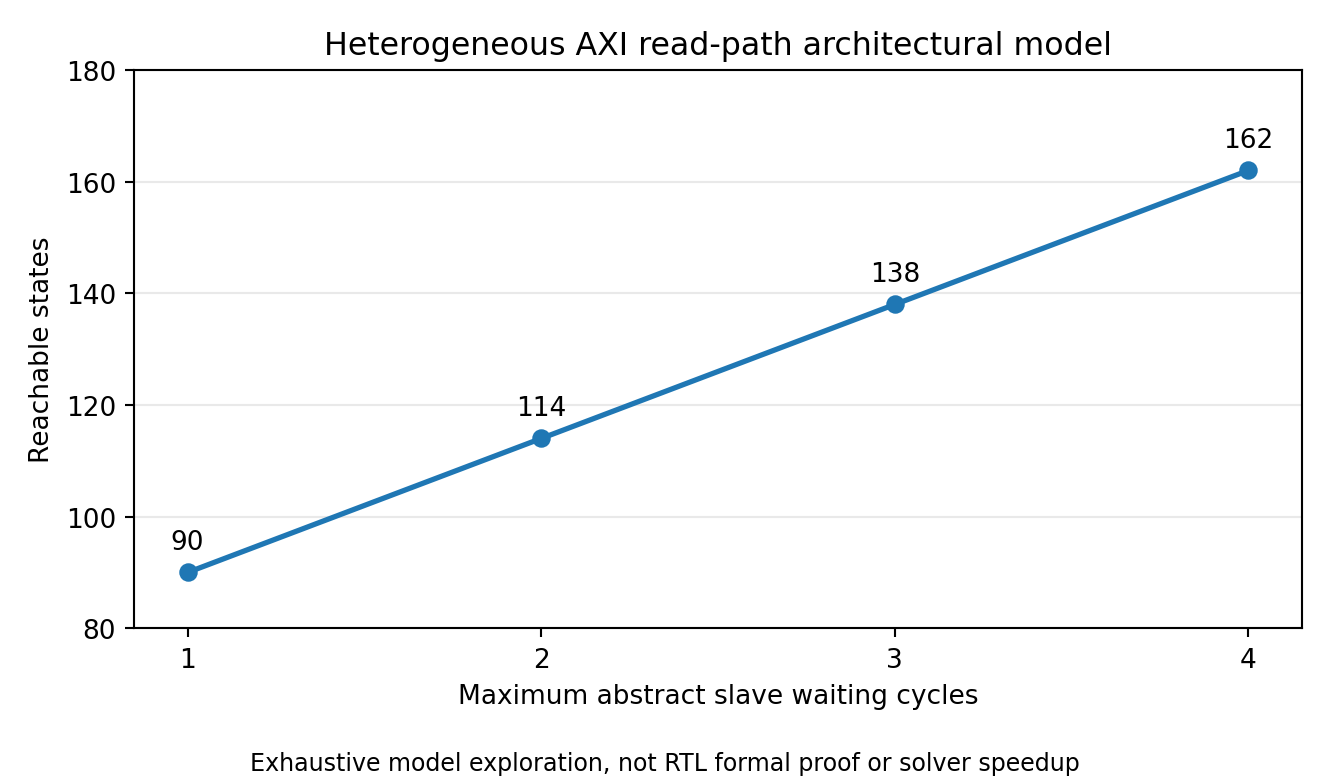
\includegraphics[width=.8\linewidth]{figures/fig1_reachable_arch_states.png}
\caption{Reachable states in the executed architectural transition system.}
\end{figure}

\begin{figure}[H]\centering
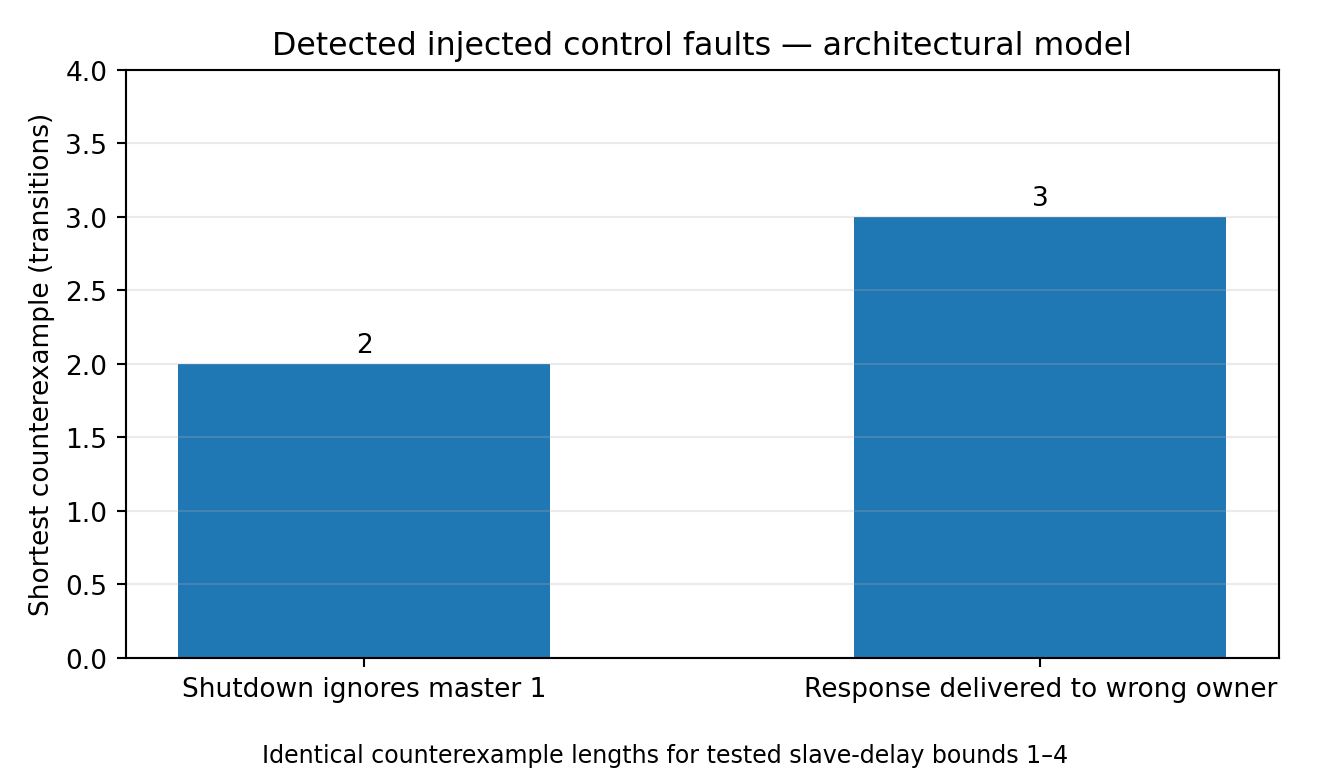
\includegraphics[width=.8\linewidth]{figures/fig2_arch_fault_witnesses.png}
\caption{Counterexample lengths for two deliberately faulty abstract designs.}
\end{figure}

\section{Independent SMT consistency checks}
Five native Z3 checks ran on explicitly stated one-step protocol-contract
relations. Three obligations returned UNSAT: credit/busy bookkeeping
inductiveness, exclusion of orphan completions under legal-credit
assumptions, and shutdown safety under correct occupancy bookkeeping. Two
negative controls returned SAT: a shutdown guard ignoring master 1 and
an erroneous response-owner case. These checks are \emph{not} evidence that
the imported interconnect implements those assumptions.

\section{Prepared external RTL test and limitations}
The package generates 12 SymbiYosys tasks over two address maps (contended and
separate), each containing a real-RTL full baseline, a standard-COI baseline,
a candidate control-contract model, two injected failures, and coverage.
The runner captures the exact upstream commit SHA, source hashes, AIG latch/AND
counts, wall times, solver outcomes, and witness VCDs. The \texttt{master}
reference is resolved and recorded during the first GitHub run; rerun with that
full SHA to pin the version.

\textbf{Assurance boundary.} The execution environment has no Yosys or
SymbiYosys and cannot fetch the upstream repository. Therefore none of the
12 RTL tasks has been proved locally. The contract candidate has no complete
verified trace-inclusion/refinement proof: its PASS, if obtained later,
\emph{must not} be represented as approval of the upstream design. Solver
UNKNOWN/timeout, missing source, and missing witness evidence fail closed.
The experiment omits AXI-Lite writes, multi-clock CDC, analog timing,
peripheral firmware, and liveness guarantees.

\textbf{Reproduction.} Extract the ZIP at the root of the existing GitHub
repository; keep \path{.github/workflows/intent2proof-axi-hetero.yml} at the
repository root. Start the workflow ``Intent2Proof heterogeneous AXI
benchmark'' and download the artifact
\path{intent2proof-heterogeneous-axi-results}. The evidence must be
audited before adding full-RTL performance claims to the main proposal.
\end{document}
